\cotefile{150}

\scanpage{52}
Je veux revenir sur la condition b), qui peut se préciser beaucoup, si on veut utiliser à fond l'information qu'on avait dans le numéro précédent.

$b_1)$ Pour $x\in\Sigma\deleted{\unsure{(0)}}=\Sigma^{\unsure{*|<}}(0)$, les $z_\alpha\in\Sigma^{<}(1)$ au dessus de $x$ (pour l'application \uline{but} : $\Sigma^{<}(1)\overset{\uline{b}}{\unsure{-|\longrightarrow}}\Sigma^{<}(0)$) sont en correspondance biunivoque avec les germes \inserted{$B_\alpha$} en $x$ de sous-espaces bordants de $\Sigma^{<}(0)$, \deleted{\unsure{avec}} images par $\uline{b}$ des germes de $\Sigma^{<}(1)$ en \deleted{\unsure{les}} $z_\alpha$.

$b_2)$ \deleted{Il existe un} Si $n=\operatorname{card}(\{z_\alpha\})$, il existe un élément \deleted{\unsure{d}} unique de $\Sigma^{<}(n)$, soit $\widetilde{x}$, tel que les \deleted{$\unsure{B_\alpha|z_\alpha}$} $z_\alpha$ soient les images de $\widetilde{x}$ par \inserted{les $n$ applications} de $\widetilde\Sigma(n)$ dans $\widetilde\Sigma(1)$.
\margin{\diagram{\begin{tikzcd}[column sep=large]
\unsure{\widetilde\Sigma^{<}(n)}\arrow[r,phantom,"{\substack{\cdot\\\cdot}}"{description,pos=0.26,yshift=-2.5ex}]\arrow[r,shift left=2ex,"\varphi_{0,n}"]\arrow[r,"\varphi_{1,n}" description]\arrow[r,shift right=2ex,"\varphi_{n-1,n}"']&\widetilde\Sigma^{*}(1)\arrow[d,phantom,"{\rotatebox{90}{$\in$}}" description]\\
&z_\alpha
\end{tikzcd}}}
(Il en résulte qu'il y a une \uline{structure d'ordre} \inserted{\uline{total}} \uline{naturelle} sur l'ens des ``strates de niveau 1'' $B_\alpha$ \inserted{dans $\Sigma^{<}(0)=\Sigma$} passant par $x$)

\deleted{\unsure{$b_2)$}} $b_3)$ Pour tout \deleted{$1\leq d\leq n$, \unsure{les}} $1\leq d\leq n$, considérons l'application
\[
\Sigma^{<}(d)\underset{\substack{\inserted{\text{imm}}\\\deleted{\unsure{\text{vigueur}}}}}{\longrightarrow}\underset{\substack{\rotatebox{90}{$\in$}\\x}}{\Sigma^{<}(0)}
\]
associée à l'inclusion \deleted{\unsure{de de}} $\{d\}\subset\{0,1,--,d\}$, les pts \inserted{$z$} de $\Sigma^{<}(d)$ au dessus de $x$ sont en correspondance biunivoque avec l'ens des parties \inserted{de card $d$} de un \deleted{$\unsure{\Sigma}$} $I$ des germes $B_\alpha$, ou encore l'ens des parties \inserted{de card $d$} de l'ens $I$ des $z_\alpha$, ou encore avec $\mathcal P_d([0,--,n-1])$, en associant : à telle partie $A$ l'application \inserted{str} croissante unique de $\Delta_d=\{0,--d\}$ en

% Lighter-hand foliation at the lower-left corner, not authorial numbering.
\margin{\handwritten{51}}

\scanpage{53}
\mspage{22}
$\Delta_n=\{0,-,n\}$ dont l'image soit $A\cup\{n\}$, et l'hom simplicial correspondant
\diagram{\begin{tikzcd}[column sep=small]
\Sigma^{<}(n)\arrow[r,hook,"\mathrm{imm}"]\arrow[d,phantom,"{\rotatebox{90}{$\in$}}" description]&\Sigma^{<}(d)\arrow[d,phantom,"{\rotatebox{90}{$\in$}}" description]&\deleted{\unsure{(\longrightarrow}}&\big(\arrow[r,dashed,"\mathrm{imm}"]&\Sigma^{<}(0)\big)\arrow[d,phantom,"{\rotatebox{90}{$\in$}}" description]\\
\widetilde x&z\ \deleted{\unsure{z}}&&&x
\end{tikzcd}}
\diagram{\begin{tikzcd}
\deleted{x}\arrow[r,phantom,"\deleted{\longleftarrow}" description]&\deleted{\unsure{\Sigma(0)}}
\end{tikzcd}}
et l'image de $\widetilde x$ par celui-ci. De plus, pour $z$ dans \deleted{ainsi} $\Sigma^{<}(d)$ au dessus de $x$, $\deleted{\unsure{Z|z}}$ le germe de sous-espace de $\Sigma^{<}(0)$ en $x$, image du germe de $\Sigma^{<}(d)$ en $z$, est juste l'intersection des germes $B_\alpha$ \unsure{correspondant|correspondants} aux $z_\alpha\in A$.

On s'intéresse ici aux morphismes entre les $\Sigma^{<}(n)$ correspondant aux applications strictement croissantes d'ens. tot\textsuperscript{t} ordonnés non vides $d\hookrightarrow d'$ tel que $d$ soit cofinal dans $d'$. La catégorie de ces objets et morphismes équivaut à celle des ens tot. ordonnés $d$ (év.\textsuperscript{t} vides), par le foncteur qui à un tel $d$ associe $d\coprod\{\omega\}$, où $\omega$ est un ``dernier élément'', et à tout $d'\hookrightarrow d$ str. croiss le prolongement par $\omega\mapsto\omega$. On a donc \deleted{\unsure{$\Sigma$}} un foncteur
\[
\Gamma:d-\Sigma^{<}(d\coprod\{\omega\})
\]
sur les ens \unsure{tot.|tot} ordonnés év.\textsuperscript{t} vides, dont la
% Cancelled interline beneath « donnée équivaut à celle… »; its attachment/revision order is not established.
\begin{tabular}[t]{@{}l@{}}
donnée équivaut à celle des $\Sigma^{<}(n)$ avec les\\
\deleted{\unsure{qui équivaut à}}
\end{tabular}
appl. simpliciales ``cofinales'' entre eux. Et la donnée d'\deleted{F}un tel foncteur $\Gamma$ revient à la donnée de $\Gamma(\varnothing)$ (ici $\Sigma^{\unsure{*|<}}(0)$) et
% Pale pencil foliation at the lower left, in another hand.
\margin{52}

\scanpage{54}
d'un objet (espace) simplicial --- \uline{dessus de}
$\Gamma(\varnothing)=\Sigma^{<}(0)$. Ici il s'agit d'un espace
\margin{NB $\Gamma(n)=\Sigma^{*}(n+1)$}
simplicial relatif, et les conditions $b_1,b_2,b_3$
concernent cette structure --- elles disent
essentiellement que cette structure est associée
à une stratification cylindrique locale de
$\Sigma^{<}(0)=\Sigma$, et ``ordonnée'' (i.e. l'ens des
strates de codim $1$ passant par un $x\in\Sigma$ sont
\deleted{\unsure{est}} \unsure{ordonnés|ordonnées}, et cette relation d'ordre varie
continûment avec $x$ en un sens évident).

Les \deleted{$\Sigma^{<}(d)$ \unsure{s'id|s'ident}} $\Gamma(d)$\inserted{$=\Sigma^{<}(d+1)$} s'identifient alors
aux \deleted{parties} espaces des \inserted{(germes de)} strates de codim
$d+1$, \deleted{les} \inserted{germes} identifiés \deleted{(grâce à la structure
d'ordre)} aux ens de germes de strates
de codim $1$ \deleted{\unsure{de}} \inserted{\unsure{en un}} $=$ $x$. Les applic\unsure{ns}
semi-simpliciales entre les $\Gamma(d)$ proviennent
alors de la structure d'ordre --- \deleted{\unsure{on y}}
\unsure{pour|peut} réconstituer les espaces de drapeaux
associés à la stratification, à l'aide des
\deleted{\unsure{cette|ces}} $\Gamma(d)$, grâce à cette structure ordonnée.
En résumé, la donnée de $\Gamma:d\mathrel{\mid\! -\!}\Gamma(d)$
\deleted{\unsure{i.e. de}} (i.e. de $\Sigma^{<}$ avec les \unsure{ap|app} \unsure{semi|\deleted{semi}} simpliciales
cofinales) équivaut à celle d'un $\Sigma=\Sigma^{<}(0)$,
\margin{53}

\scanpage{55}
\mspage{23}
avec la structure de stratification cylindrique \inserted{ordonnée}
locale. \deleted{Par exemple}, Une autre façon de
décrire les $\Gamma(d)=\Sigma^{<}(d+1)$, c'est de
prendre la puiss. \deleted{\unsure{sym.}} \inserted{cart. relative} $d$.ième de $\Gamma_0$\deleted{\unsure{$(\varnothing)$}}\inserted{$=\Sigma^{<}(1)$}
sur $\Sigma\ (=\Gamma(\varnothing))$, dont on enlève les images
des puiss. cart. relatives \deleted{\unsure{inférieures}} \inserted{\deleted{$\Gamma'(d)$} des $d'$.ième ($d'<d$)} par les applic\unsure{ns}
$\tfrac12$ simpliciales entre celles ci. Cela donne à priori
les \deleted{\unsure{ens tot.}} suites ordonnées de $d$ germes de
strates de codim $1$ \inserted{en un $=$ point,} \unsure{(mutuel\textsuperscript{t}|\deleted{(mutuel\textsuperscript{t}}} distinctes), \deleted{soit}
$\Gamma'(d)$. On a alors \inserted{$\unsure{\Gamma^{\deleted{'}}(d)|\Gamma(d)}\subset\Gamma'(d)$},
$\Gamma(d)$ est une partie à la fois ouverte et
\unsure{fermée|\deleted{fermée}} de $\Gamma'(d)$, et \deleted{$\Gamma'(d)\unsure{\simeq}$}
\[
(35)\qquad \Gamma'(d)\simeq\unsure{\mathfrak S_d|\mathcal S_d}\times\Gamma(d)
\]
Pour avoir \deleted{la}\inserted{une} structure d'ordre \inserted{total} relative, de
\margin{\deleted{il s'agit de}}
\deleted{\unsure{$\Gamma'(1)$ sur}} $\Gamma_0=\Sigma^{<}(1)$ sur $\Sigma_{\deleted{\unsure{*|0}}}=\Sigma^{<}(0)$, il \deleted{suffit}\inserted{\unsure{uniquement}}
de se donner, \deleted{dans $\Gamma'_1(\unsure{0|2})=\unsure{\Sigma^{<}(0)|\Sigma^{<}(2)}$, $\Gamma'_{1+1}$} dans
$\Gamma_0\times_\Sigma\Gamma_0\setminus\text{diagonale}$, une partie \inserted{(i.e. \unsure{néc.}} ouverte et fermée)
$\Gamma_1$, telle que $\Gamma_1\cup{}^s\Gamma_1=\Gamma_0\times\Gamma_0\setminus\text{diag}$, $\Gamma_1\cap{}^s\Gamma_1=\varnothing$
\margin{$\Gamma_1$ est le graphe de la relation $x<y$}
i.e. une section de $\Gamma_0\times_\Sigma\Gamma_0\setminus\text{diag}$ \unsure{au|\deleted{au}} dessus
\margin{ou une section \deleted{de $\Gamma_0\times_\Sigma\Gamma_0\setminus\unsure{\text{diagonale}|\text{diag}}$}\deleted{de $\operatorname{Sym}^2(\Gamma_0\times_\Sigma\Gamma_0)$}\deleted{de}}
de $\operatorname{Sym}^2_\Sigma(\Gamma_0)^*$ (``choix d'un premier élément parmi deux
éléments distincts), avec la condition de transitivité
\deleted{$\unsure{\text{que }\Gamma_1}$}
\diagram{\begin{tikzcd}[column sep=large,row sep=small]
(36)\quad (\Gamma_1\times_\Sigma\Gamma_0)\cap(\Gamma_0\times_\Sigma\Gamma_1)
 \arrow[r,"{\unsure{\operatorname{Pr}|\mathrm{P}}_{\unsure{13|23}}}"] \arrow[d,phantom,"\cap" description]
 & \Gamma_0\times\Gamma_0 \arrow[d,phantom,"\cup" description]
 & \text{se factorise par }\Gamma_1 \\
\unsure{\Sigma_0|\Gamma_0}\times\Gamma_0\times\Gamma_0 & \Gamma_1 &
\end{tikzcd}}
\margin{54}

\scanpage{56}
Je m'aperçois finalement que j'ai
pas mal bousillé pour arriver à trouver des
formulations simples --- car j'ai \uline{mélangé} des
propriétés purement ensemblistes de l'ens ordonné
$\Sigma=\Sigma^{<}(0)$, avec \unsure{\deleted{leur}|leur} interprétation semi-simpliciale,
et \deleted{\unsure{leur} \illegible{1}}\inserted{les} aspects topologiques. Je \uline{reprends}

\deleted{$\Sigma$ ens.}
% Detached pen marks, without a secure textual function: [307,869,327,885],
% [350,877,369,884], [422,886,459,901]; isolated stroke [939,773,949,790].
$\underset{\substack{\Vert\\\Sigma(0)}}{\Sigma}$ ens ordonné, muni d'une topologie \deleted{séparée}\inserted{(pour}
Si $\Sigma_1$ est le graphe de la relation d'ordre, on suppose

\textcircled{a} $\Sigma(1)\xrightarrow{\uline{b}\unsure{=|:}\operatorname{pr}_2}\Sigma(0)$ est propre et loc. immersif bordant
\unsure{\inserted{(propriétés topologiques)}|(propriétés topologiques)} \deleted{Cela implique}

\deleted{\textcircled{b}} \deleted{que l'applic\unsure{ati|ation}}
Cela implique que l'application diagonale est
ouverte, donc si $\Sigma$ séparé, son image est une
partie à la fois ouverte et fermee --- et on
peut alors introduire $\Sigma_F^{\unsure{<|*}}(1)=\Sigma(1)\setminus\text{diagonale}$.
Si $\Sigma$ est séparé, la propreté de $\Sigma(1)-\Sigma(0)$
implique aussi que $\Sigma_1$ est \uline{fermé} dans \deleted{$\Sigma(0)\times\Sigma(0)$}\inserted{$\Sigma\times\Sigma$}.

\textcircled{b} Pour tt $x\in\Sigma$, l'ens \inserted{(fini)} $\Sigma_{\leq x}$ \inserted{(fibre de $x$ dans $\Sigma(1)$)} est \uline{tot. ordonné}
pour l'ordre induit.
\deleted{\textcircled{\unsure{c}}} Donc la donnée d'un drapeau \inserted{$x_{i_0}-x_{\unsure{j_d|i_d}}$} de longueur
$d$ dans $\Sigma_\leq$ équivaut à celle d'une partie de card. $d+1$

% Lighter-hand foliation at the lower-left corner.
\margin{\handwritten{55}}

\scanpage{57}
\mspage{24}
de l'ens à $N(x)+1$ éléments, où $N(x)=\operatorname{card}(\Sigma_{\unsure{<|\leq}x})$.
Ou encore, si on regarde l'application-but
\[
\Sigma^{<}(d)\longrightarrow\unsure{\Sigma}=\Sigma^{<}(0)
\]
\[
(x_0<-<x_d)\longmapsto x_d
\]
la fibre de $x\in\Sigma$ s'identifie à l'ens \deleted{des parties}
$\unsure{\mathfrak P|\mathcal P}_d(\{1,.-,N(x)\})$.
La structure relative de $\Sigma^{\unsure{<|*}}(1)$ sur $\Sigma=\Sigma^{<}(0)$
% Isolated dark written sign directly below the bare middle Sigma, between
% this line and the next: two short forked left strokes joined to a compact
% loop or oval at the right. Identity and mathematical attachment unassigned.
\illegible{1}
est donc celle d'un ens tot. ordonné relatif, qui
permet de reconstituer le système des $\Sigma^{*}(d)$
\deleted{avec} $(d\in\mathbb N)$ avec les applications semi-simpliciales
correspondant aux morphismes cofinaux entre
les ens tot. ordonnés-types.
% Slanted marginal note beside the preceding three lines; its words are
% not an insertion after semi-simpliciales. The final circled character is unclear.
\margin{Tout ceci est donc à faire indépendt de toute condition topologique \unsure{\textcircled{a}}.}

\textcircled{c} $\forall\ x\in\Sigma$, les germes \inserted{$B_\alpha$} de sous-espaces \inserted{bordants} de $\Sigma$ en $x$
correspondants, par \unsure{\textcircled{a}}, aux $z_\alpha\in\Sigma^{\unsure{<|*}}(1)$ au dessus
de $x$ (par $\Sigma^{\unsure{<|*}}(1)\overset{\underline b}{\unsure{-|\longrightarrow}}\Sigma$) sont mutuellement transver-
saux (et à fortiori distincts).
Les germes intersections de certains des $B_\alpha$
correspondent donc aux pts des $\Sigma^{\unsure{<|*}}(d)$ au dessus
de $x$ (par $\Sigma^{\unsure{<|*}}(d)\overset{\underline b}{\relbar\joinrel\relbar}\Sigma$), comme
images du \deleted{\unsure{dit}} germe de $\Sigma^{\unsure{<|*}}(d)$ en ces pts.
% Separate cancelled small looped glyph immediately before Les; no letter assigned.
\deleted{\illegible{1}} Les espaces $\Sigma^{*}(d)$ $(d\in\mathbb N)$ et les
applications $\tfrac12$ simpliciales cofinales entre eux, \deleted{\unsure{satisfa}}
% In the preceding cancellation a small final loop follows the tall f;
% its reading as a remains doubtful, and the abandoned word is not completed.
ou encore l'espace relatif $\Sigma^{\unsure{<|*}}(1)$ sur $\Sigma^{<}(0)$ et la
structure d'ordre relative, est décrit entièrement
% Pale bottom-left foliation, apparently another hand; the top authorial number is 24.
\margin{56}

\scanpage{58}
par $\Sigma$, muni d'une stratification locale
cylindrique ordonnée : $\Sigma'(1)$ est l'espace des
strates de codim $1$, $\Sigma'(1)\overset{\uline{b}}{-}\Sigma\unsure{{}_{0}|.}$ l'application
associant à un germe son centre, $\Sigma'(2)$ est
l'espace des paires de germes $B,B'$ en $x$
\deleted{\unsure{que}} tels que : $\{B\}<\{B'\}$ \unsure{\illegible{1}..|...}
\margin{\diagram{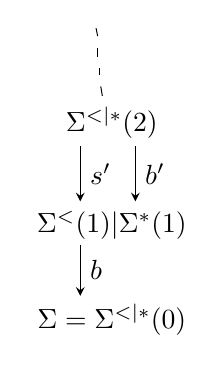
\begin{tikzpicture}[x=1cm,y=1cm,>=stealth]
\draw[line width=.35pt] (-.2,1.65)--(-.18,1.55);
\draw[line width=.35pt] (-.18,1.4)--(-.18,1.28);
\draw[line width=.35pt] (-.16,1.14)--(-.16,1.06);
\draw[line width=.35pt] (-.14,.91)--(-.12,.79);
\node at (0,.45) {$\Sigma^{\unsure{<|*}}(2)$};
\node at (0,-.85) {$\unsure{\Sigma^{<}(1)|\Sigma^{*}(1)}$};
\node at (0,-2.05) {$\Sigma=\Sigma^{\unsure{<|*}}(0)$};
\draw[->] (-.4,.15)--(-.4,-.55) node[midway,right] {$\uline{s}'$};
\draw[->] (.3,.15)--(.3,-.55) node[midway,right] {$\uline{b}'$};
\draw[->] (-.4,-1.1)--(-.4,-1.75) node[midway,right] {$\uline{b}$};
\end{tikzpicture}}}
Pour retrouver la relation d'ordre sur $\Sigma\unsure{=|\substack{-\\0}}\Sigma^{\unsure{<|*}}(0)$
\inserted{à partir de la structure d'ordre relative $\Sigma^{\unsure{*|<}}(1)$ sur $\Sigma^{<}(0)$ (celle
qui \unsure{place} $\Sigma^{<}(1)$ pour les relations strictes $x<y$)}
il faut donc de plus se donner une application
continue
\[
(36)\qquad\Sigma^{<}(1)\overset{\uline{s}\unsure{=|:}p_1}{-}\Sigma_{\deleted{\unsure{*|\varnothing|0}}}=\Sigma^{<}(0)
\]
qui soit injective \deleted{et croissante} sur chaque fibre \inserted{$\uline{b}^{-1}(x)$}
de $\Sigma^{<}(1)\overset{\uline{b}}{-}\Sigma_{\deleted{\unsure{*|\varnothing|0}}}$ (i.e. $\Sigma^{<}(1)\overset{(\uline{s},\uline{b})}{-}\Sigma\times\Sigma$ inj.)
et d'image $\not\ni x$ (i.e. $\operatorname{Im}(\uline{s},\uline{b})\cap\operatorname{diag}(\Sigma\times\Sigma)=\varnothing$)

\deleted{et on doit se donner de plus
\[
(37)\qquad\Sigma^{<}(2)\xrightarrow{\unsure{\varphi_2|p_2}}\Sigma^{*}(1)\quad(\hookrightarrow\Sigma\times\Sigma
\]
\margin{NB la donnée de $\unsure{\varphi_2|p_2}$ équivaut à celle des deux composés
$\operatorname{pr}_{\unsure{0|1}}\circ\varphi;\operatorname{pr}_{\unsure{1|2}}\circ\varphi:\Sigma^{<}(2)\rightrightarrows\Sigma$
qu'on \unsure{se} donne}
\margin{inutile de se donner $p_2$, il est déterminé ($v\ p_1$), cf \unsure{pg} suivante\unsure{.-|..|...}}
\[
(38)\qquad
\Sigma^{<}(2)\xrightarrow{(\operatorname{pr}_1\circ\varphi,\operatorname{pr}_2\circ\varphi,\unsure{\Psi|\psi})}\Sigma_0\times\Sigma_0\times\Sigma_0
\]
\unsure{\deleted{Dont}|Dont} l'image est par construction (voir \unsure{\deleted{\varphi}|\varphi|\illegible{1}} (37))
dans $\Sigma_1\times\Sigma_0$ et dans
}
\margin{\handwritten{57}}

\scanpage{59}
\mspage{\unsure{\{25\}}}
de telle façon qu'il existe
\[
(37)\qquad p_2:\Sigma^{<}(2)\longrightarrow\Sigma^{\unsure{<|*}}(1)
\]
tel que
\[
(38)\qquad \left\{\begin{aligned}
\uline{b}\circ p_2&=\uline{s}\circ\uline{b'}\\[6em]
p_1\circ p_2&=p_1\circ\uline{s'}
\end{aligned}\right.
\]
i.e. le carré
\diagram{\begin{tikzcd}[row sep=large,column sep=large,name=s59square,execute at end picture={
\coordinate (s59ha) at ([xshift=10pt]s59sourcea.east);
\fill ([yshift=6pt]s59ha) circle[radius=.45pt];
\draw[line width=.7pt,line cap=round] ([xshift=-1.5pt,yshift=5.5pt]s59ha)--([xshift=-2.5pt,yshift=5pt]s59ha);
\draw[line width=.7pt,line cap=round] ([xshift=-3pt,yshift=4.3pt]s59ha)--([xshift=-3.4pt,yshift=3.4pt]s59ha);
\draw[line width=.7pt,line cap=round] ([xshift=-3.8pt,yshift=2.7pt]s59ha)--([xshift=-3.7pt,yshift=2pt]s59ha);
\draw[line width=.7pt,line cap=round] ([xshift=-3.2pt,yshift=1.2pt]s59ha)--([xshift=-2.6pt,yshift=.4pt]s59ha);
\coordinate (s59hb) at ([xshift=10pt]s59sourceb.east);
\fill ([yshift=6pt]s59hb) circle[radius=.45pt];
\fill ([xshift=-1.8pt,yshift=6.1pt]s59hb) circle[radius=.5pt];
\fill ([xshift=-3.7pt,yshift=4.7pt]s59hb) circle[radius=.55pt];
\fill ([xshift=-4.8pt,yshift=3.2pt]s59hb) circle[radius=.55pt];
\draw[line width=.8pt,line cap=round] ([xshift=-5pt,yshift=1.3pt]s59hb)--([xshift=-4.2pt,yshift=.3pt]s59hb);
\fill ([yshift=4pt]s59targetd.north) circle[radius=.9pt];
}]
|[alias=s59sourcea]|\Sigma^{<}(2)\arrow[r,"\uline{b'}",start anchor=east,shorten <=10pt]\arrow[d,"p_2"] & \Sigma^{<}(1)\arrow[d,"p_1=\uline{s}",dash,end anchor=north,shorten >=4pt]\\
|[alias=s59sourceb]|\Sigma^{<}(1)\arrow[r,"\uline{b}",start anchor=east,shorten <=10pt] & |[alias=s59targetd]|\Sigma
\arrow[ul,phantom,"\text{(cart)}" description]
\end{tikzcd}}
commutatif
\figure{\begin{tikzpicture}[x=1cm,y=1cm]
\draw[line width=.45pt,line cap=round] (0,0)
.. controls (.65,-.02) and (.90,.02) .. (1.08,.13)
-- (1.30,.50)
.. controls (1.55,.72) and (1.70,.77) .. (1.90,.76)
.. controls (2.70,.70) and (3.50,.81) .. (4.90,.77);
\end{tikzpicture}}

i.e. le carré
\diagram{\begin{tikzcd}[name=s59diamond,execute at end picture={
\coordinate (s59hc) at ([xshift=-6pt,yshift=6pt]s59sourcec.north west);
\draw[line width=.7pt,line cap=round] ([xshift=-4.5pt,yshift=2pt]s59hc)--([xshift=-4.2pt,yshift=1pt]s59hc);
\draw[line width=.7pt,line cap=round] ([xshift=-2.8pt]s59hc)--([xshift=-1.7pt,yshift=-.2pt]s59hc);
\fill (s59hc) circle[radius=.5pt];
\draw[line width=.7pt,line cap=round] ([xshift=2pt,yshift=.8pt]s59hc)--([xshift=2.8pt,yshift=1.5pt]s59hc);
}]
& \Sigma^{<}(1)\arrow[dl,"p_1"'] & \\
\Sigma && |[alias=s59sourcec]|\Sigma^{<}(2)\arrow[ul,"\uline{s'}"',start anchor=north west,shorten <=7pt]\arrow[dl,"p_2"]\\
&\Sigma^{<}(1)\arrow[ul,"p_1"]&
\end{tikzcd}}
est comm.

Ce qui détermine $p_2$ de façon unique, puisque
$(\deleted{\unsure{b}},p_1,\uline{b}):\Sigma^{<}(1)\unsure{\longrightarrow|\mathrel{-}}\Sigma\unsure{<|\times}\Sigma$ est mono).
De plus, on \deleted{\unsure{suppose}}\inserted{doit} exiger que le premier carré
(38) soit \uline{cartésien}, et que $p_1:\Sigma^{<}(1)\unsure{\longrightarrow|\mathrel{-}}\Sigma$
est \uline{transversal} p.r. à l'immersion bordante
$\uline{b}:$ \diagram{\begin{tikzcd}[column sep=large,execute at end picture={
\coordinate (s59hi) at ([xshift=9pt]s59inline.east);
\draw[line width=.65pt,line cap=round] ([yshift=6pt]s59hi)--([xshift=-1.4pt,yshift=5.8pt]s59hi);
\draw[line width=.65pt,line cap=round] ([xshift=-3pt,yshift=5pt]s59hi)--([xshift=-4.2pt,yshift=4.3pt]s59hi)--([xshift=-5pt,yshift=2.8pt]s59hi)--([xshift=-4.4pt,yshift=1.3pt]s59hi)--([xshift=-3pt,yshift=.4pt]s59hi);
\fill ([xshift=-1.5pt]s59hi) circle[radius=.4pt];
}]
|[alias=s59inline]|\Sigma^{<}(1)\arrow[r,"\uline{b}",start anchor=east,shorten <=9pt]&\Sigma
\end{tikzcd}} (ce qui est \deleted{\unsure{une}}\inserted{l'unique} condition de
nature non purement algébrique\ldots)
Posons alors, pour $x,y\in\Sigma$
\[
(39)\qquad x\prec y\quad\Longleftrightarrow\quad\exists\ u\in\Sigma_{<}(1)\text{ tel que }x=p_1u,\ y=\uline{b}u
\]
\margin{58}

\scanpage{60}
On voit alors que
\[
x\prec y\text{ et }y\prec z\quad\Longrightarrow\quad x\prec z
\]
car soient $u,v\in\Sigma_{\unsure{<|*}}(1)$ tels que
\[
\mathord{\rlap{$\deleted{\unsure{s}}$}p}_1 u=x,\quad\uline{b}u=\underbrace{y,\quad p_1}v=y,\quad\uline{b}v=z
\]
% In the first glyph the possible cancelled s overlaps the head of p;
% the earlier letter is unresolved. The short brace is spatial: it lies
% beneath the first y toward the following p_1, not beneath both complete equalities.
on a donc
\[
\unsure{\uline{b}}u=p_1v
\]
% This b and its underline are heavily overdrawn. No earlier character is assigned.
donc par le carré cartésien de (38), \deleted{$\exists\unsure{w|u}$}
\[
\exists\mid\ d\in\Sigma^{\unsure{<|*}}(2),\quad\text{avec}\quad\uline{b'}(d)=v,\quad p_2(d)=u
\]
soit
\[
w=\uline{s'}(d)\in\Sigma^{\unsure{<|*}}(1)
\]
on a
\[
\begin{aligned}
p_1(w)&=p_1(\uline{s'}(d))\overset{(38)}{=}p_1p_2(d)=p_1(u)=x\\
\uline{b}(w)&=\uline{b}(\uline{s'}(d))=\uline{b}(\uline{b'}(d))=\uline{b}(v)=z
\end{aligned}
\]
donc
\figure{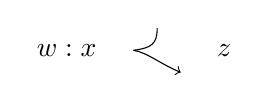
\begin{tikzpicture}[baseline=(x.base)]
\node (x) at (0,0) {$w:x$};
\node at (2,0) {$z$};
\draw (1.15,.28) .. controls (1.15,.08) and (1.08,.03) .. (.85,0);
\draw[->] (.85,0) .. controls (1.03,-.03) and (1.2,-.18) .. (1.45,-.28);
\end{tikzpicture}}.
De plus, on a
\[
x\not\prec x\qquad\left(\text{car }\operatorname{Im}(\Sigma_1\overset{(p_1;\uline{b})}{\relbar\joinrel\relbar}\Sigma\times\Sigma)\cap\text{diag}=\varnothing\right)
\]
% The final = empty-set and the end of the parenthesis continue below at the right.
donc la relation $x\prec y$ est la relation
d'inégalité stricte associée à une relation
d'ordre sur $\Sigma$. On récupère $\Sigma^{\unsure{<|*}}(1)$ comme
le graphe de la relation d'ordre stricte,
$\Sigma^{<}(2)$ comme les drapeaux $x\prec y\prec z$ de
longueur $2$ dans \illegible{1} $\Sigma$, et les applications
% A separate small curved upright is raised in the gap after dans, before Sigma;
% its value is unassigned. It is preserved above as an unread fragment.
% Pale lower-left foliation, apparently another hand; no top authorial number is visible.
\margin{59}

\scanpage{62}
b) L'application $\Sigma^{<}(2)\xrightarrow{(p_1\circ s',\unsure{p_1b'|p_1\circ b'})}\Sigma\times\Sigma$
se factorise par $\Sigma^{<}(1)\lhook\joinrel\xrightarrow{(p_1,\uline{b})}\Sigma\times\Sigma$
en un morphisme
\[
p_2:\Sigma^{<}(2)-\Sigma^{<}(1)
\]
qui rende le carré
\diagram{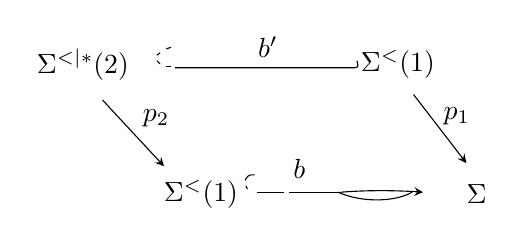
\begin{tikzpicture}[x=1cm,y=1cm,>=stealth]
\node at (0,0) {$\Sigma^{\unsure{<|*}}(2)$};
\node at (4,0) {$\Sigma^{<}(1)$};
\node at (1.5,-1.65) {$\Sigma^{<}(1)$};
\node at (5,-1.65) {$\Sigma$};
% Four separated upper hook fragments.
\draw[line width=.4pt] (1.12,.22)--(1.06,.20);
\draw[line width=.4pt] (.98,.15)--(.94,.12);
\draw[line width=.4pt] (.94,.05)--(.98,.01);
\draw[line width=.4pt] (1.05,-.02)--(1.12,-.02);
% Unheaded upper shaft, with its upturned endpoint.
\draw (1.17,-.04)--(3.45,-.04) .. controls (3.5,-.04) and (3.5,-.01) .. (3.48,.05);
\node at (2.35,.22) {$\uline{b}'$};
\draw[->] (.25,-.45)--(1.03,-1.29);
\node at (.93,-.68) {$p_2$};
\draw[->] (4.2,-.38)--(4.87,-1.25);
\node at (4.75,-.65) {$p_1$};
% Two lower hook fragments, short first shaft segment, and a gap.
\draw (2.18,-1.40) .. controls (2.10,-1.39) and (2.08,-1.43) .. (2.06,-1.47);
\draw[line width=.4pt] (2.07,-1.54)--(2.09,-1.58);
\draw (2.21,-1.62)--(2.55,-1.62);
\draw (2.62,-1.62)--(3.28,-1.62);
% The rightward portion is retraced into an elongated open loop.
\draw[->] (3.28,-1.62) .. controls (3.65,-1.59) and (4.02,-1.60) .. (4.32,-1.62);
\draw (3.24,-1.62) .. controls (3.58,-1.77) and (4.00,-1.73) .. (4.18,-1.62);
\node at (2.75,-1.32) {$\uline{b}$};
\end{tikzpicture}}
\uline{Cartésien}, et $p_1:\Sigma^{<}(1)-\Sigma$ étant transversal
à \deleted{\unsure{l'imm}}ersion-but $\uline{b}:\Sigma^{\unsure{<|*}}(1)-\Sigma$.
\margin{\uline{NB} (Si $\Sigma$ est séparé, donc $\Sigma\times\Sigma$ séparé
sur $\Sigma$, et $\Sigma^{<}(1)\overset{\uline{b}}{-}\Sigma$
propre, il en résulte
que $\Sigma^{<}(1)-\Sigma\times\Sigma$ est
propre donc un plongement
\uline{fermé}.}
\margin{cette condition de transversalité est
peut être conséquence des autres .-}

De façon équivalente, une telle structure
est donnée par un espace topologique \inserted{séparé} $\Sigma$,
muni d'une relation d'ordre $x\preceq y$
\deleted{dont le graphe est}\inserted{satisfaisant les conditions suivantes}

% Two unassigned dark points beside the first cancelled a) line.
\margin{\figure{\begin{tikzpicture}[x=1mm,y=1mm]
\fill (0,0) circle (.16mm);
\fill (.5,-.8) circle (.16mm);
\end{tikzpicture}}}
\deleted{a) le graphe \deleted{$\unsure{\Sigma^{<}(1)|\Sigma^{*}(1)}$} $\Sigma(1)$ de cette relation est
fermé dans $\Sigma\times\Sigma$, et $\Sigma(1)\overset{\uline{b}}{-}\Sigma$ est
une immersion\unsure{.}
\deleted{$\unsure{\Sigma}$}
b) Si $\Sigma^{*}(1)$ est le graphe de la
relation d'ordre \inserted{stricte}, $\Sigma^{*}(1)\xrightarrow{\uline{b}}\Sigma$ est une
immersion \inserted{bordante} propre \deleted{\unsure{(donc la partie de}}
a) Si $x\in\Sigma$, $\Sigma_{<x}$ \inserted{$(=\Sigma^{\unsure{<|*}}(1)_{\unsure{x}})$}\unsure{,}
\unsure{\deleted{\unsure{est} \unsure{un|une}}|\unsure{est} \unsure{un|une}}
\unsure{ens|est} (fini) \uline{tot}$ {}^t$. \uline{ordonné}.
}
\margin{\handwritten{61}}

\scanpage{63}
\mspage{27}
\deleted{c) Si $(z_\alpha)_{\alpha\in I}$ est l'ens des éléments de
$\Sigma_{<x}=\uline{b}^{-1}(\{x\})$ (où $\uline{b}:\Sigma^{\unsure{<|*}}(1)\longrightarrow\Sigma$), les
\unsure{les};}

a) Pour \unsure{tt|$\forall$} $x\in\Sigma$, l'ens $\Sigma_{<x}$ \deleted{(fini) \unsure{est}}\inserted{est tot${}^t$}
\deleted{$\simeq\uline{b}^{-1}(\{x\}$} ordonné

b) Si $\Sigma^{\unsure{*|<}}(1)$ est le graphe de la relation
$x<y$, et $\uline{s},\uline{b}:\Sigma^{<}(1)\unsure{\rightrightarrows|=}\Sigma$ sont les applications
source et but, \deleted{\illegible{1}} l'application $\uline{b}$ est une immer-
sion \deleted{\uline{\unsure{bordante}}} \uline{propre} (donc les $\Sigma_{<x}\unsure{\ne|=}\uline{b}^{-1}(\{x\})$
sont finis)

c) Si $(z_\alpha)_{\alpha\in I}$ sont les éléments de $\Sigma_{<x}=b^{-1}(\{x\})$,
alors \inserted{la famille} \unsure{des|les} \unsure{g}ermes \inserted{en $x$} de sous-espaces \deleted{\unsure{bordants}}\inserted{de $\Sigma$}
images par $\uline{b}$ des \inserted{germes} $(\Sigma^{<}(1),z_\alpha)$, est \inserted{une famille}
\deleted{\unsure{transversaux}}\inserted{transversale}
de sous-espaces \uline{bordants}.

d) $\uline{\unsure{b|s|p_1}}:\Sigma^{<}(1)\longrightarrow\Sigma^*$ est \uline{transversal} p.r. à l'immersion
bordante $\uline{b}:\Sigma^{<}(1)\mathrel{-}\Sigma^{\unsure{*}}$
\deleted{\unsure{la diag.}}
\margin{ou sous forme d'une \unsure{récollection|récollement}
pour les $z_\alpha\in\Sigma^{<}(1)$ au dessus d'un même
$x\in\Sigma^*$\ldots}

$1^{\circ})$ Cas équisingulier : $\uline{s}:\Sigma^{<}(1)\mathrel{-}\Sigma$ fibrant \inserted{(propre)}

$2^{\circ})$ Cas non singulier : $\unsure{\Sigma}$ est une variété à bord,
dont le bord est $\uline{b}(\Sigma^{*}(1))$:

$3^{\circ})$ Cas \unsure{équisingulier|équi-singulier}-non-singulier : $\uline{s}:\Sigma^{<}(1)\mathrel{-}\Sigma$ est
fibrant \inserted{propre}, à fibres des variétés à bord, et le
fibré des bords est l'image de $\Sigma^{*}(2)$ par
le morphisme $\Sigma^{*}(2)\xrightarrow{\uline{s'}}\Sigma^{\unsure{*|<}}(1)$ \deleted{\unsure{avec}}\inserted{donné}
par $(x\prec y\prec z)\longrightarrow(x\prec z)$.
\margin{c'est sans doute conséquence de la conjonction des deux conditions $1^{\circ}),2^{\circ})$}
\margin{62}

\scanpage{64}
Les morphismes les plus importants dans la
situation apparaissent dans le diagramme
% The curved leader attaches hexagonal immediately before the live suivant.
\inserted{hexagonal} suivant
\diagram{\begin{tikzcd}[column sep=9mm,row sep=13mm,arrows={line width=.6pt},execute at end picture={
% Upper b: four separate hook components, with unequal lengths.
\draw[line width=.7pt,line cap=round] ([xshift=7.1pt,yshift=6.0pt]s64upper.east) -- ([xshift=8.6pt,yshift=6.6pt]s64upper.east);
\draw[line width=.6pt,line cap=round] ([xshift=5.3pt,yshift=4.6pt]s64upper.east) -- ([xshift=4.6pt,yshift=3.6pt]s64upper.east);
\draw[line width=.6pt,line cap=round] ([xshift=4.3pt,yshift=2.5pt]s64upper.east) .. controls +(0pt,-1.5pt) and +(-1pt,0pt) .. ([xshift=5.4pt,yshift=.8pt]s64upper.east);
\draw[line width=.6pt,line cap=round] ([xshift=6.4pt,yshift=.5pt]s64upper.east) .. controls +(.5pt,.2pt) and +(-.5pt,0pt) .. ([xshift=7.6pt,yshift=.8pt]s64upper.east);
% Central b-prime: four components; the second one is visibly faint.
\draw[line width=.6pt,line cap=round] ([xshift=7.2pt,yshift=6.2pt]s64centre.east) -- ([xshift=8.2pt,yshift=6.8pt]s64centre.east);
\draw[line width=.4pt,black!45,line cap=round] ([xshift=5.9pt,yshift=5.3pt]s64centre.east) -- ([xshift=5.2pt,yshift=4.5pt]s64centre.east);
\draw[line width=.6pt,line cap=round] ([xshift=4.4pt,yshift=3.3pt]s64centre.east) .. controls +(0pt,-1.5pt) and +(-.2pt,.5pt) .. ([xshift=4.4pt,yshift=1.6pt]s64centre.east);
\draw[line width=.6pt,line cap=round] ([xshift=5.3pt,yshift=1.0pt]s64centre.east) -- ([xshift=7.1pt,yshift=.6pt]s64centre.east);
% Upper-right b: three detached pieces at the source.
\draw[line width=.6pt,line cap=round] ([xshift=-8.7pt,yshift=4.8pt]s64right.north west) .. controls +(-.7pt,.9pt) and +(0pt,-.5pt) .. ([xshift=-9.1pt,yshift=6.0pt]s64right.north west);
\draw[line width=.6pt,line cap=round] ([xshift=-8.0pt,yshift=3.8pt]s64right.north west) -- ([xshift=-6.7pt,yshift=3.1pt]s64right.north west);
\draw[line width=.6pt,line cap=round] ([xshift=-5.6pt,yshift=3.0pt]s64right.north west) .. controls +(.6pt,0pt) and +(-.4pt,-.4pt) .. ([xshift=-4.5pt,yshift=3.5pt]s64right.north west);
% Lower b: one detached upper curl, and one lower bend joined to the shaft.
\draw[line width=.7pt,line cap=round] ([xshift=4.7pt,yshift=4.1pt]s64lower.east) .. controls +(0pt,1pt) and +(-.8pt,.4pt) .. ([xshift=6.4pt,yshift=5.3pt]s64lower.east);
\draw[line width=.6pt,line cap=round] ([xshift=4.0pt,yshift=2.4pt]s64lower.east) .. controls +(-.2pt,-2.6pt) and +(-2pt,0pt) .. ([xshift=7pt]s64lower.east);
% s-prime: two unequal visible shafts merge at one head.  Its source curl
% comprises a long U-like part and a separate right arc, with a pen gap.
\draw[->,line width=.85pt,line cap=round] ([xshift=-2.5pt,yshift=8.0pt]s64centre.north west) -- ([yshift=-2pt]s64upper.south east);
\draw[line width=.5pt,line cap=round] ([xshift=.8pt,yshift=9.1pt]s64centre.north west) .. controls +(-3pt,4pt) and +(4pt,-3pt) .. ([yshift=-2pt]s64upper.south east);
\draw[line width=.7pt,line cap=round] ([xshift=-10pt,yshift=7pt]s64centre.north west) .. controls +(0pt,-3pt) and +(-2pt,0pt) .. ([xshift=-3.5pt,yshift=4.5pt]s64centre.north west) .. controls +(1.5pt,0pt) and +(0pt,-1.3pt) .. ([xshift=-2pt,yshift=6.3pt]s64centre.north west);
\draw[line width=.6pt,line cap=round] ([xshift=-.8pt,yshift=5.1pt]s64centre.north west) .. controls +(2.1pt,.6pt) and +(1pt,-1pt) .. ([xshift=1.2pt,yshift=8.0pt]s64centre.north west);
\node[anchor=east] at ([xshift=-18mm,yshift=3pt]s64left.west) {$(40)$};
\node[anchor=west] at ([xshift=34mm,yshift=-3mm]s64bottom.east) {,};
}]
&|[alias=s64upper]|\Sigma^{\unsure{<|*}}(1)\arrow[rr,"\uline{b}",start anchor=east,shorten <=9pt]\arrow[dl,"\uline{s}"']&&|[alias=s64top]|\Sigma&\\
|[alias=s64left]|\Sigma&&|[alias=s64centre]|\Sigma^{*}(2)\arrow[ul,phantom,"\uline{s'}"']\arrow[rr,"\uline{b}'",start anchor=east,shorten <=9pt]\arrow[dl,"\uline{p}"']\arrow[ur,phantom,"\text{cart}" description]\arrow[dr,phantom,"\text{cart}" description]&&|[alias=s64right]|\Sigma^{\unsure{<|*}}(1)\arrow[ul,"\uline{b}"',start anchor=north west,shorten <=7pt]\arrow[dl,"\uline{s}"]\\
&|[alias=s64lower]|\Sigma^{\unsure{<|*}}(1)\arrow[ul,"\uline{s}"']\arrow[rr,"\uline{b}",start anchor=east,shorten <=7pt]&&|[alias=s64bottom]|\Sigma&
\end{tikzcd}}

où les flèches marquées \diagram{\begin{tikzcd}[column sep=large,arrows={line width=.6pt},execute at end picture={
% Four disconnected marks: an upper slant, then three short dot-like pieces.
\draw[line width=.7pt,line cap=round] ([xshift=6.3pt,yshift=6.1pt]s64legend.east) -- ([xshift=8pt,yshift=6.8pt]s64legend.east);
\fill ([xshift=5.1pt,yshift=4.8pt]s64legend.east) circle[radius=.48pt];
\fill ([xshift=5.3pt,yshift=3.1pt]s64legend.east) circle[radius=.48pt];
\fill ([xshift=6pt,yshift=1.7pt]s64legend.east) circle[radius=.43pt];}]
|[alias=s64legend]|{}\arrow[r,start anchor=east,shorten <=8pt]&{}
\end{tikzcd}} (en fait,
$\uline{b},\deleted{\unsure{p_2}},\uline{b'},\uline{s'}$) sont des immersions bordantes \inserted{propres},
% propres is above bordantes; its surrounding curve continues into the
% insertion leader, ending after bordantes before the separate comma.
et les flèches marquées $\longrightarrow$ (en fait,
$\uline{s}$ et $\uline{p}$) sont (dans le cas équisingulier)
fibrantes et propres \unsure{\}} (\unsure{voire|voir}, de plus : fibres
des variétés à bord, dont le bord est
dans le cas de $\unsure{\uline{s}|\uline{s'}}:\Sigma^{\unsure{<|*}}(1)\longrightarrow\Sigma$, l'image
% A short dark raised stroke above this s may be a pen-start or a prime;
% both readings are retained.  No identification with the later s-prime is imposed.
de $\Sigma^{\unsure{<|*}}(2)\overset{\uline{s'}}{-}\Sigma^{*}(1)$
% The initial curve before i.e. continues below the insertion and into its
% long leader.  It is not separately repeated as a literal parenthesis.
\inserted{i.e. l'ens des $(x\prec y)$ tels que $y$ \uline{ne soit pas} successeur de $x$}).
% The insertion is above this map; successeur de x wraps at its right end.
% The following note is oblique in the left margin beside the fibre/boundary passage.
\margin{donc, dans le cas de $\uline{p}:\Sigma^{\unsure{<|*}}(2)\mathrel{\unsure{-|\longrightarrow}}\Sigma^{\unsure{*|<}}(1)$,
le fibré des bords est l'image de $\Sigma^{\unsure{<|*}}(3)$}
On fera attention
que les applications fibrantes $\uline{s},\uline{p}$ n'ont \deleted{\unsure{rien}}\inserted{rien}
de surjectif --- l'image de $\unsure{\uline{s}|s}$ est formé des $x\in\Sigma$
qui \uline{ne sont pas maximaux}, celle de $p$ est formé
des $(x\prec y)$ tels que $y$ ne soit pas maximal.
% Pale bottom-left foliation, another hand; no authorial page number at the head.
\margin{63}
